%!TEX program = xelatex
\documentclass[10pt, compress]{beamer}
\usetheme[titleprogressbar]{m}
%\usetheme{CambridgeUS}

\usepackage{booktabs}
\usepackage[scale=2]{ccicons}
\usepackage{minted}
\usepackage[utf8]{inputenc}
\usepackage{lmodern}
\usepackage[spanish, mexico]{babel}
%\usepackage{color}
%\usepackage[usenames,dvipsnames,svgnames,table]{xcolor}

\usepackage{enumitem}
\setlist[itemize,1]{label={\fontfamily{cmr}\fontencoding{T1}\selectfont\textbullet}}
\setlist[itemize,2]{label=\textopenbullet}
\setlist[itemize,3]{label=\textopenbullet}

\setbeamercolor{block title}{use=structure, bg=orange!50,fg=black}
%\setbeamercolor{block title}{use=structure, bg=gray!40,fg=black}
\setbeamercolor{block body}{use=structure, bg=gray!20,fg=black}
%\setbeamercolor{structure}{fg=darkred}

\usepgfplotslibrary{dateplot}

\usemintedstyle{trac}

\title{\sc DETECCIÓN DEL ROSTRO HUMANO, ESTIMACIÓN DE SU POSE Y DE SU MIRADA}
\subtitle{Avances de Tesis}
\author{Rajiv González}
\institute{Maestría en Ciencias de la Computación, UADY}

\begin{document}

\maketitle

\begin{frame}[fragile]
	\frametitle{Introducción}
	\begin{itemize}
		\item ¿Por qué una persona mueve su cabeza?
		\item Importancia de conocer la posición y orientación
		\item Mediante imágenes capturas de personas es posible conocer la posición y orientación de su cabeza.

		\begin{figure}[htbp]
			\centering
			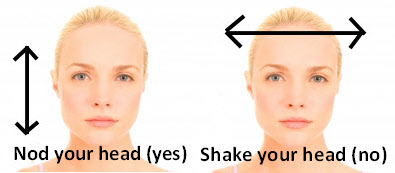
\includegraphics[width=.5\textwidth]{./pictures/nod}
		\end{figure}
	\end{itemize}

\end{frame}

\begin{frame}[fragile]
\frametitle{Objetivo}
  \begin{block}{}
  Detectar el rostro de las personas y estimar su pose mediante una cámara monocular con el objetivo de inferir la región que estén mirando en un plano virtual enfrente de ellas.
  \end{block}
\end{frame}

\begin{frame}[fragile]
\frametitle{¿Qué es la estimación de la pose de una cabeza?}
  \begin{block}{Visión computacional}
	Es el proceso de inferir la orientación y la posición de una cabeza
	humana a partir de imágenes [Murphy et al, 2009].
  \end{block}
	\begin{figure}[htbp]
		\centering
		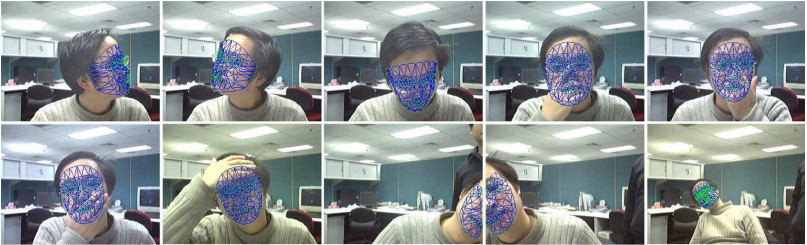
\includegraphics[width=.9\textwidth]{./pictures/pose}
	\end{figure}
\end{frame}

\begin{frame}[fragile]
	\frametitle{Aspectos a tomar en cuenta}
	 \begin{itemize}
	 	\item Previamente se debió haber localizado el rostro.
	 	\item La cabeza humana puede ser modelada como un objeto rígido.
	 	\item Marco de referencia centrado en la cámara.
	 	\item Para estimar la mirada con precisión se debe complementar con un sistema seguidor de ojos, [Wang et al, 2009].
	 \end{itemize}
	 
	 \begin{figure}[htbp] 
	 	\centering
	 	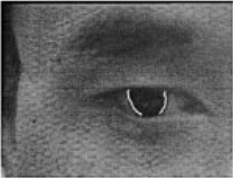
\includegraphics[width=.27\textwidth]{./pictures/gaze1}
	 	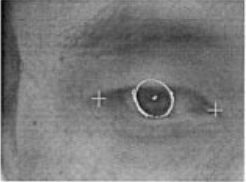
\includegraphics[width=.28\textwidth]{./pictures/gaze2}
	 	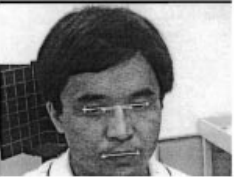
\includegraphics[width=.27\textwidth]{./pictures/gaze3}
	 \end{figure}	
\end{frame}
	


\begin{frame}[fragile]
	\frametitle{Etapas del desarrollo del proyecto de tesis}
	\begin{itemize}
		\item Localizar el rostro en la imagen
		\item Geometría del lugar de experimentación
			\begin{itemize}
				\item Relación entre la ubicación de la cabeza de la persona y la región que está observando
				\item Graficación de posibles casos
%				\item Simulación
	 	 	\end{itemize}
	 	 \item Diseño y fabricación de tarjeta de adquisición de datos
	 	 \item Algoritmo generador de mejores posiciones (puntos 3d) en la escena
	 	 \item Proyección de puntos en el plano del piso
	 	 	\begin{itemize}
	 	 		\item Descomposición de la matriz $H$ para hallar la $R$ y $T$, y el plano
	 	 		\item Optimización con Levenberg-Marquardt
	 	 		\item Reproyección de puntos e intersección con el plano
	 	 	\end{itemize}
	 	 
	 	 \item Captura de datos
	 	 \item Red Neuronal
	 	 \item Experimentos y resultados
 	 	
 	\end{itemize}
\end{frame}

\begin{frame}[fragile]
	\frametitle{Localizar rostros en la imagen}
	OpenBR
	\begin{figure}[htbp]
		\centering
		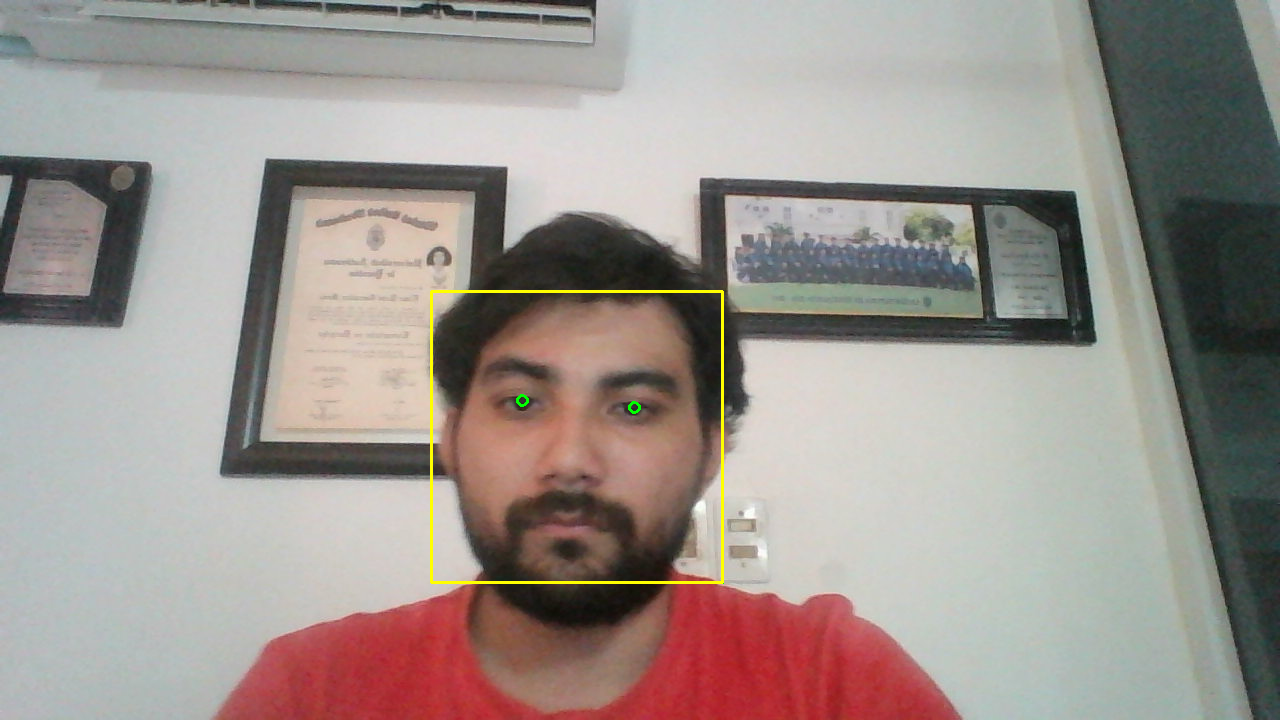
\includegraphics[width=.7\textwidth]{./pictures/detector}
	\end{figure}
\end{frame}

\begin{frame}[fragile]
\frametitle{Geometría del lugar de experimentación}
\framesubtitle{Relación entre la ubicación de la cabeza de la persona y la región que está observando}
\begin{block}{Encontrar la posición de la persona y de lo que mira en pantalla con respecto a la cámara.  Parámetros a considerar:}
	\begin{itemize}
		\item Estatura de la persona
		\item Dimensiones de la pantalla donde se desplegará la figura
		\item Distancia de la cámara a la pantalla (eje $Y$)
		\item Distancia de la pantalla(eje $Y$) al plano del piso
		
%			\begin{itemize}
%			\item Estatura de la persona con respecto al plano del piso (eje $Y$)
%			\item Distancia del de la cámara al plano del piso (eje $Y$)
%			\item Distancia del plano de la pantalla a la persona
%
%			\end{itemize}				
	\end{itemize}	
\end{block}
	 \begin{figure}[htbp] 
	 	\centering
	 	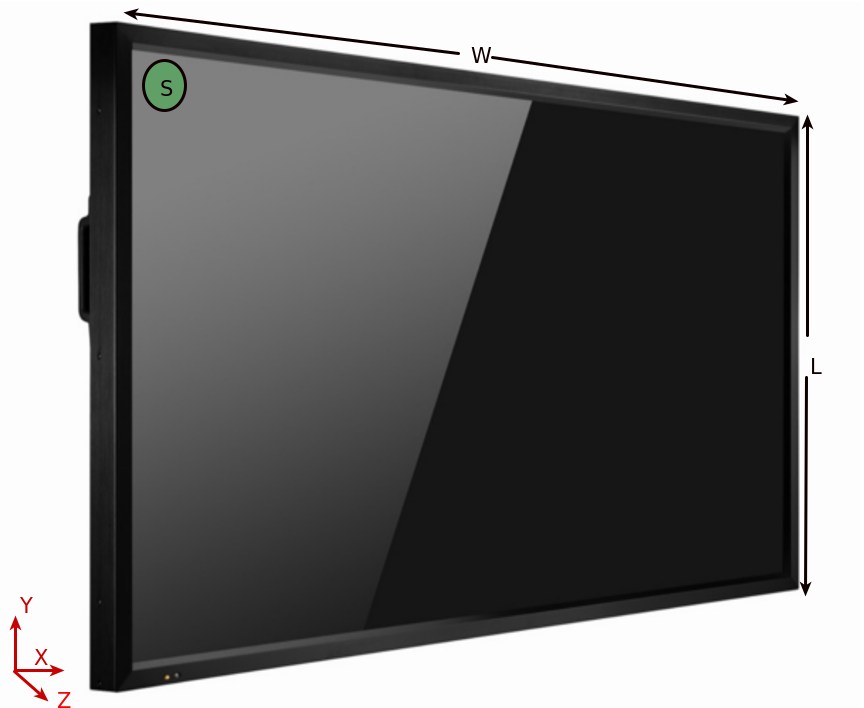
\includegraphics[width=.27\textwidth]{./pictures/pantalla2}
	 	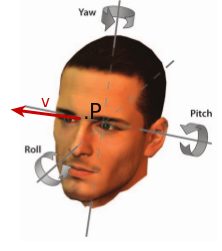
\includegraphics[width=.28\textwidth]{./pictures/personaMirando}
	 \end{figure}
\end{frame}
\begin{frame}[fragile]
	\frametitle{Geometría del lugar de experimentación}
	\framesubtitle{Relación entre la ubicación de la cabeza de la persona y la región que está observando}
		 \begin{figure}[htbp] 
		 	\centering
		 	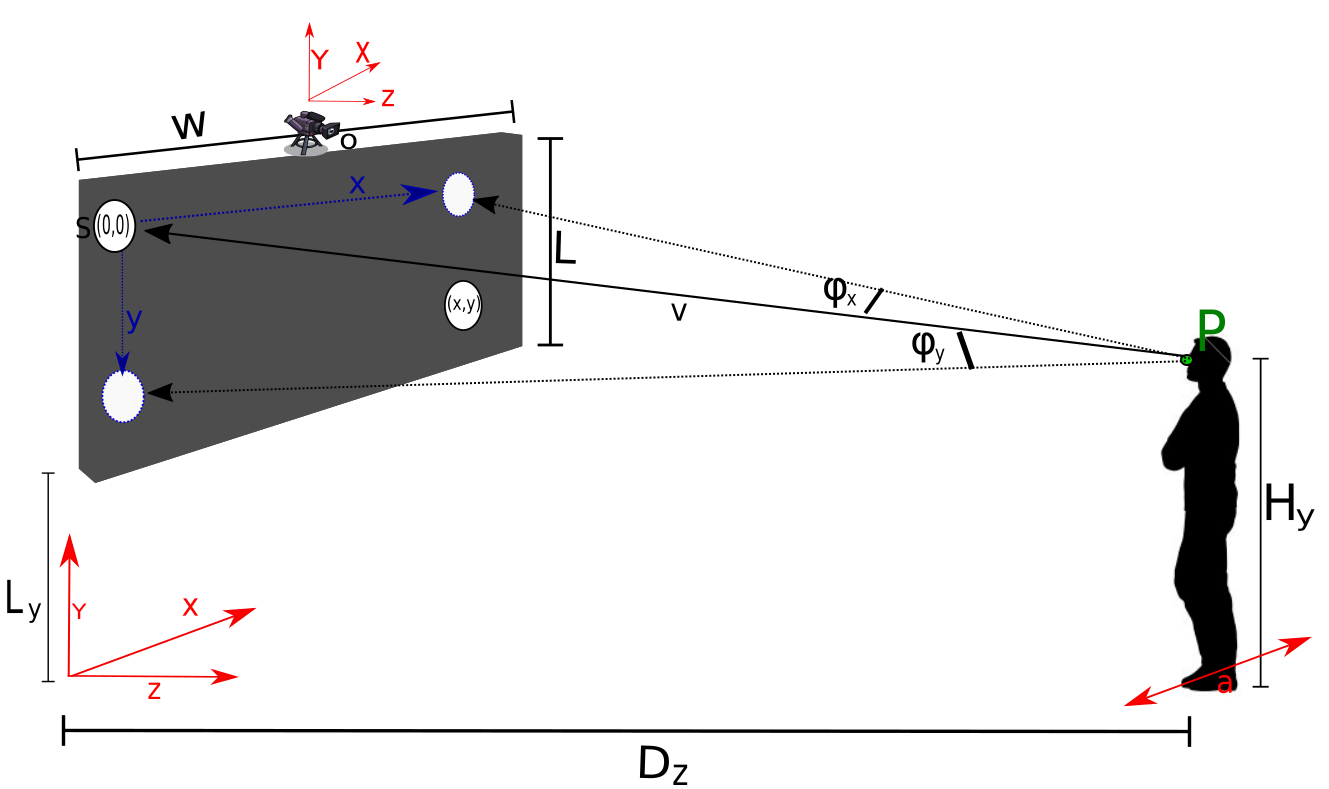
\includegraphics[width=.85\textwidth]{./pictures/escenario}
		 \end{figure}
		 \begin{eqnarray}
		 S= [S_x, S_y, S_z]^T= [x-W/2, -(c_y+y), 0]^T
		 \end{eqnarray}
		 \begin{eqnarray}
		 P=[P_x, P_y, P_z]^T= [a, -(L_y+L-H_y), D_z]^T
		 \end{eqnarray}
\end{frame}	

\begin{frame}[fragile]
	\frametitle{Geometría del lugar de experimentación}
	%\framesubtitle{Ecuaciones que describen el desplazamiento}
	\begin{itemize}
		\item 	Ecuaciones que describen el desplazamiento de la figura en pantalla y la mirada de la persona: $\phi_x y \phi_y$
		\item Cosenos directores
		%Cosenos directores de un vector a – son cosenos de ángulos que forma el vector con positivos semiejes de coordinadas.
		%Se llaman Cosenos directores del vector Å a los cosenos de los ángulos que forman cada uno de los ejes coordenados. En un plano tridimensional se representan:
	\end{itemize}
		 \begin{figure}[htbp] 
		 	\centering
		 	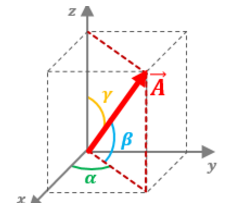
\includegraphics[width=.2\textwidth]{./pictures/directores}
		 \end{figure}
		 
		 {\small\begin{eqnarray}
		 cos(\phi_y)=\frac{\vec v_y}{|\vec v|}\\
		 cos(\phi_x)=\frac{\vec v_x}{|\vec v|}\\
		 \phi_y=cos^{-1} (\frac{-c_y-y+(L_y+L-H_y)}{\sqrt{(x-\frac{W}{2}-a)^2+(-c_y-y+(L_y+L-H_y))^2+(-D_z)^2}})\\
		 \phi_x=cos^{-1}(\frac{x-\frac{W}{2}-a}{\sqrt{(x-\frac{W}{2}-a)^2+(-c_y-y+(L_y+L-H_y))^2+(-D_z)^2}})
		 \end{eqnarray}}
\end{frame}	

\begin{frame}[fragile]
	\frametitle{Geometría del lugar de experimentación}
	\framesubtitle{Graficación de posibles casos}
		 \begin{figure}[htbp]
		 	\centering
		 	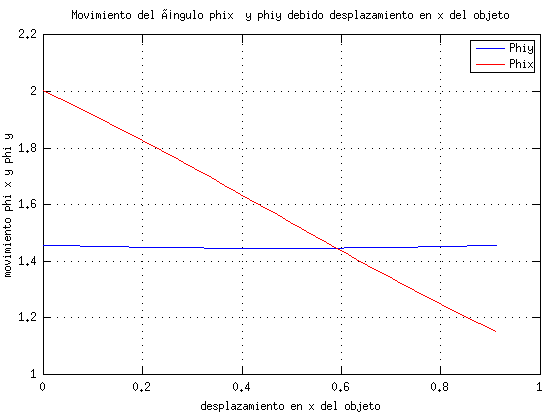
\includegraphics[width=0.4\textwidth]{./pictures/figure1}
		 	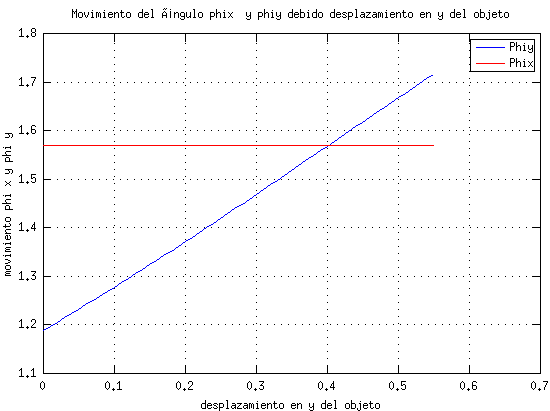
\includegraphics[width=0.4\textwidth]{./pictures/figure2}
		 \end{figure}
		 \begin{figure}[htbp]
		 	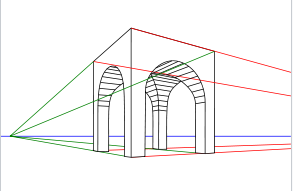
\includegraphics[width=0.4\textwidth]{./pictures/fuga}
		 \end{figure}
		 	
\end{frame}	

\begin{frame}[fragile]
	\frametitle{Geometría del lugar de experimentación}
	\framesubtitle{Graficación de posibles casos}
	\begin{figure}[htbp]
	 	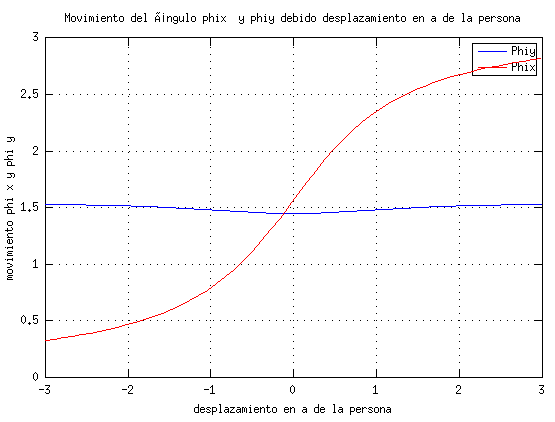
\includegraphics[width=0.4\textwidth]{./pictures/figure3}
	 	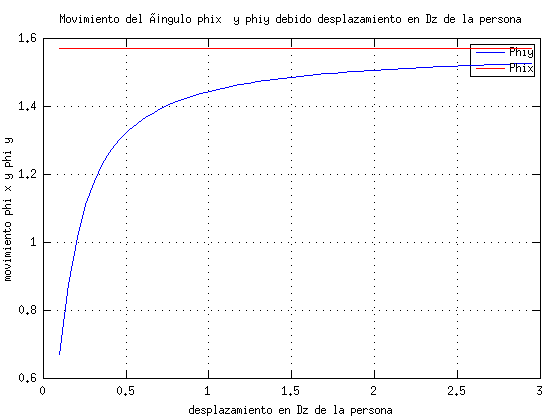
\includegraphics[width=0.4\textwidth]{./pictures/figure4}
	\end{figure}

	\begin{figure}[htbp]
	 	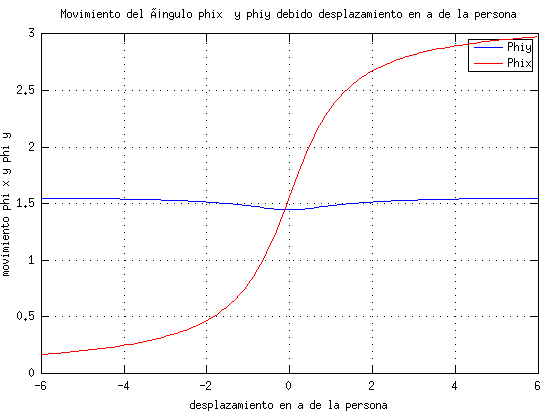
\includegraphics[width=0.4\textwidth]{./pictures/figure5}
	\end{figure}
\end{frame}	

\begin{frame}[fragile]
	\frametitle{Tarjeta de adquisición de datos}
	\begin{figure}[htbp]
		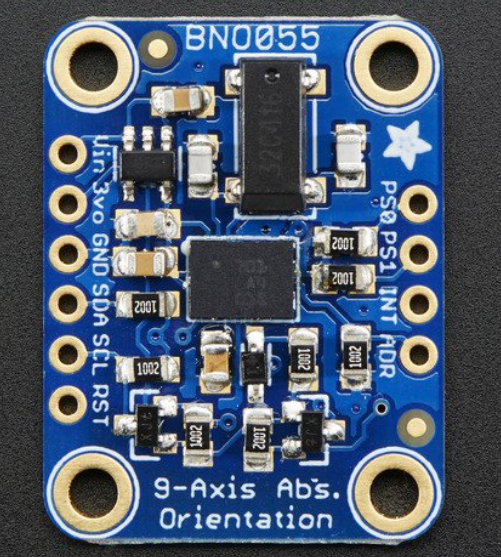
\includegraphics[width=0.1\textwidth]{./pictures/bno055}
		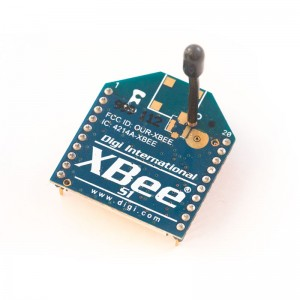
\includegraphics[width=0.2\textwidth]{./pictures/xbee}
	\end{figure}
	\begin{figure}[htbp]
		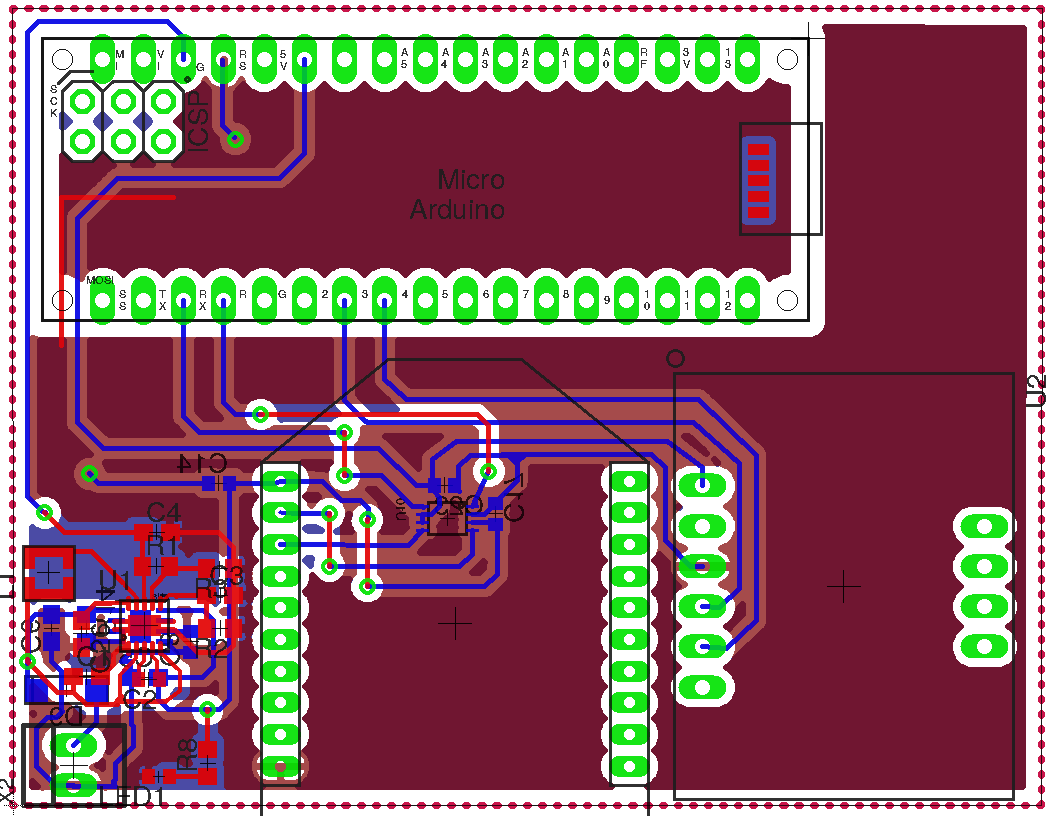
\includegraphics[width=0.4\textwidth]{./pictures/board}
		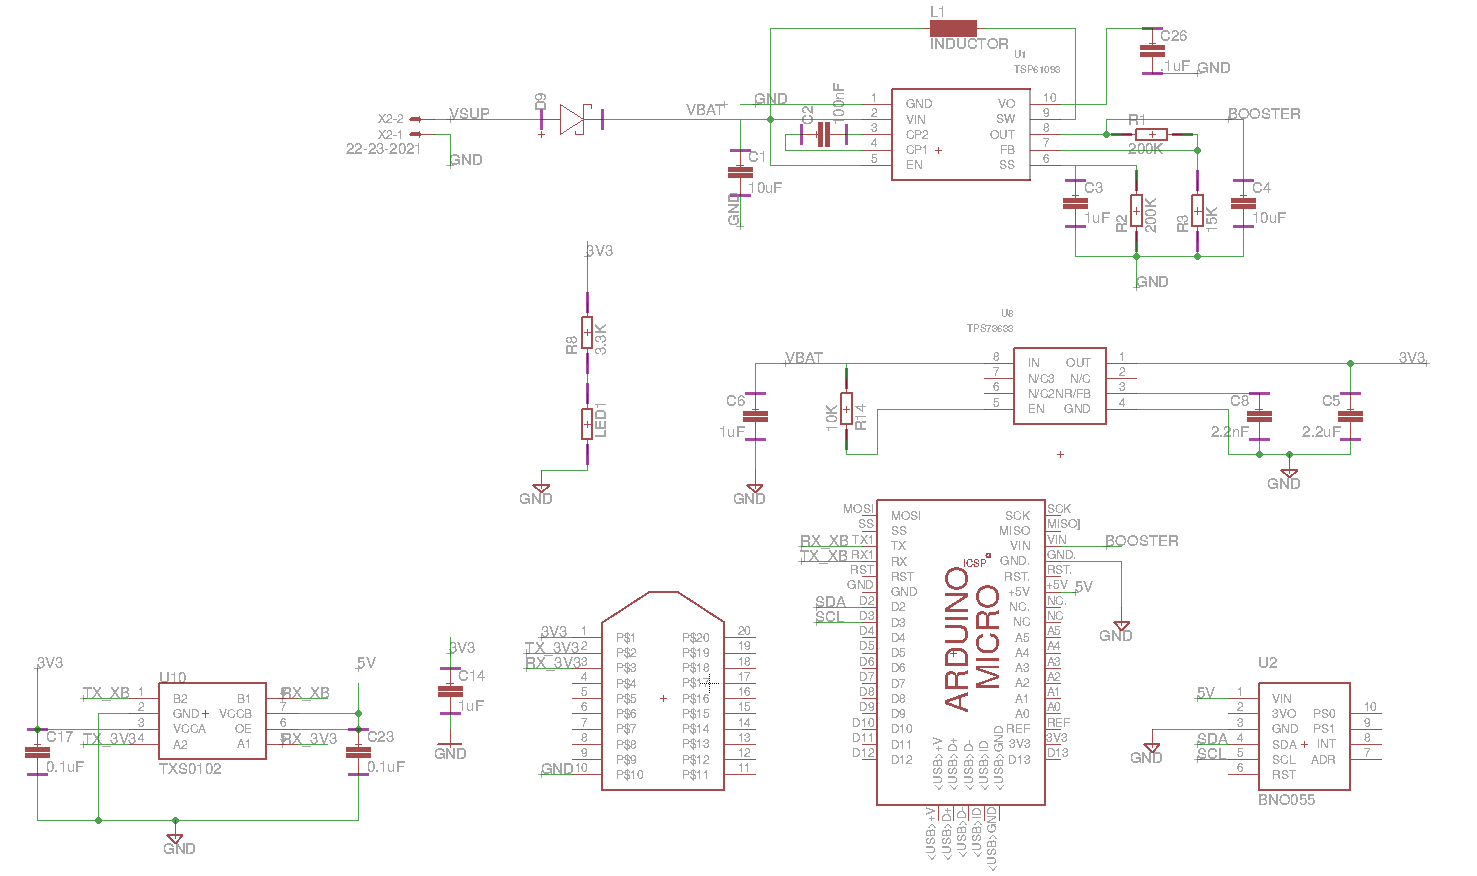
\includegraphics[width=0.6\textwidth]{./pictures/schematic}
	\end{figure}
	
\end{frame}	

\begin{frame}[fragile]
	\frametitle{Tarjeta de adquisición de datos}
	\begin{figure}[htbp]
		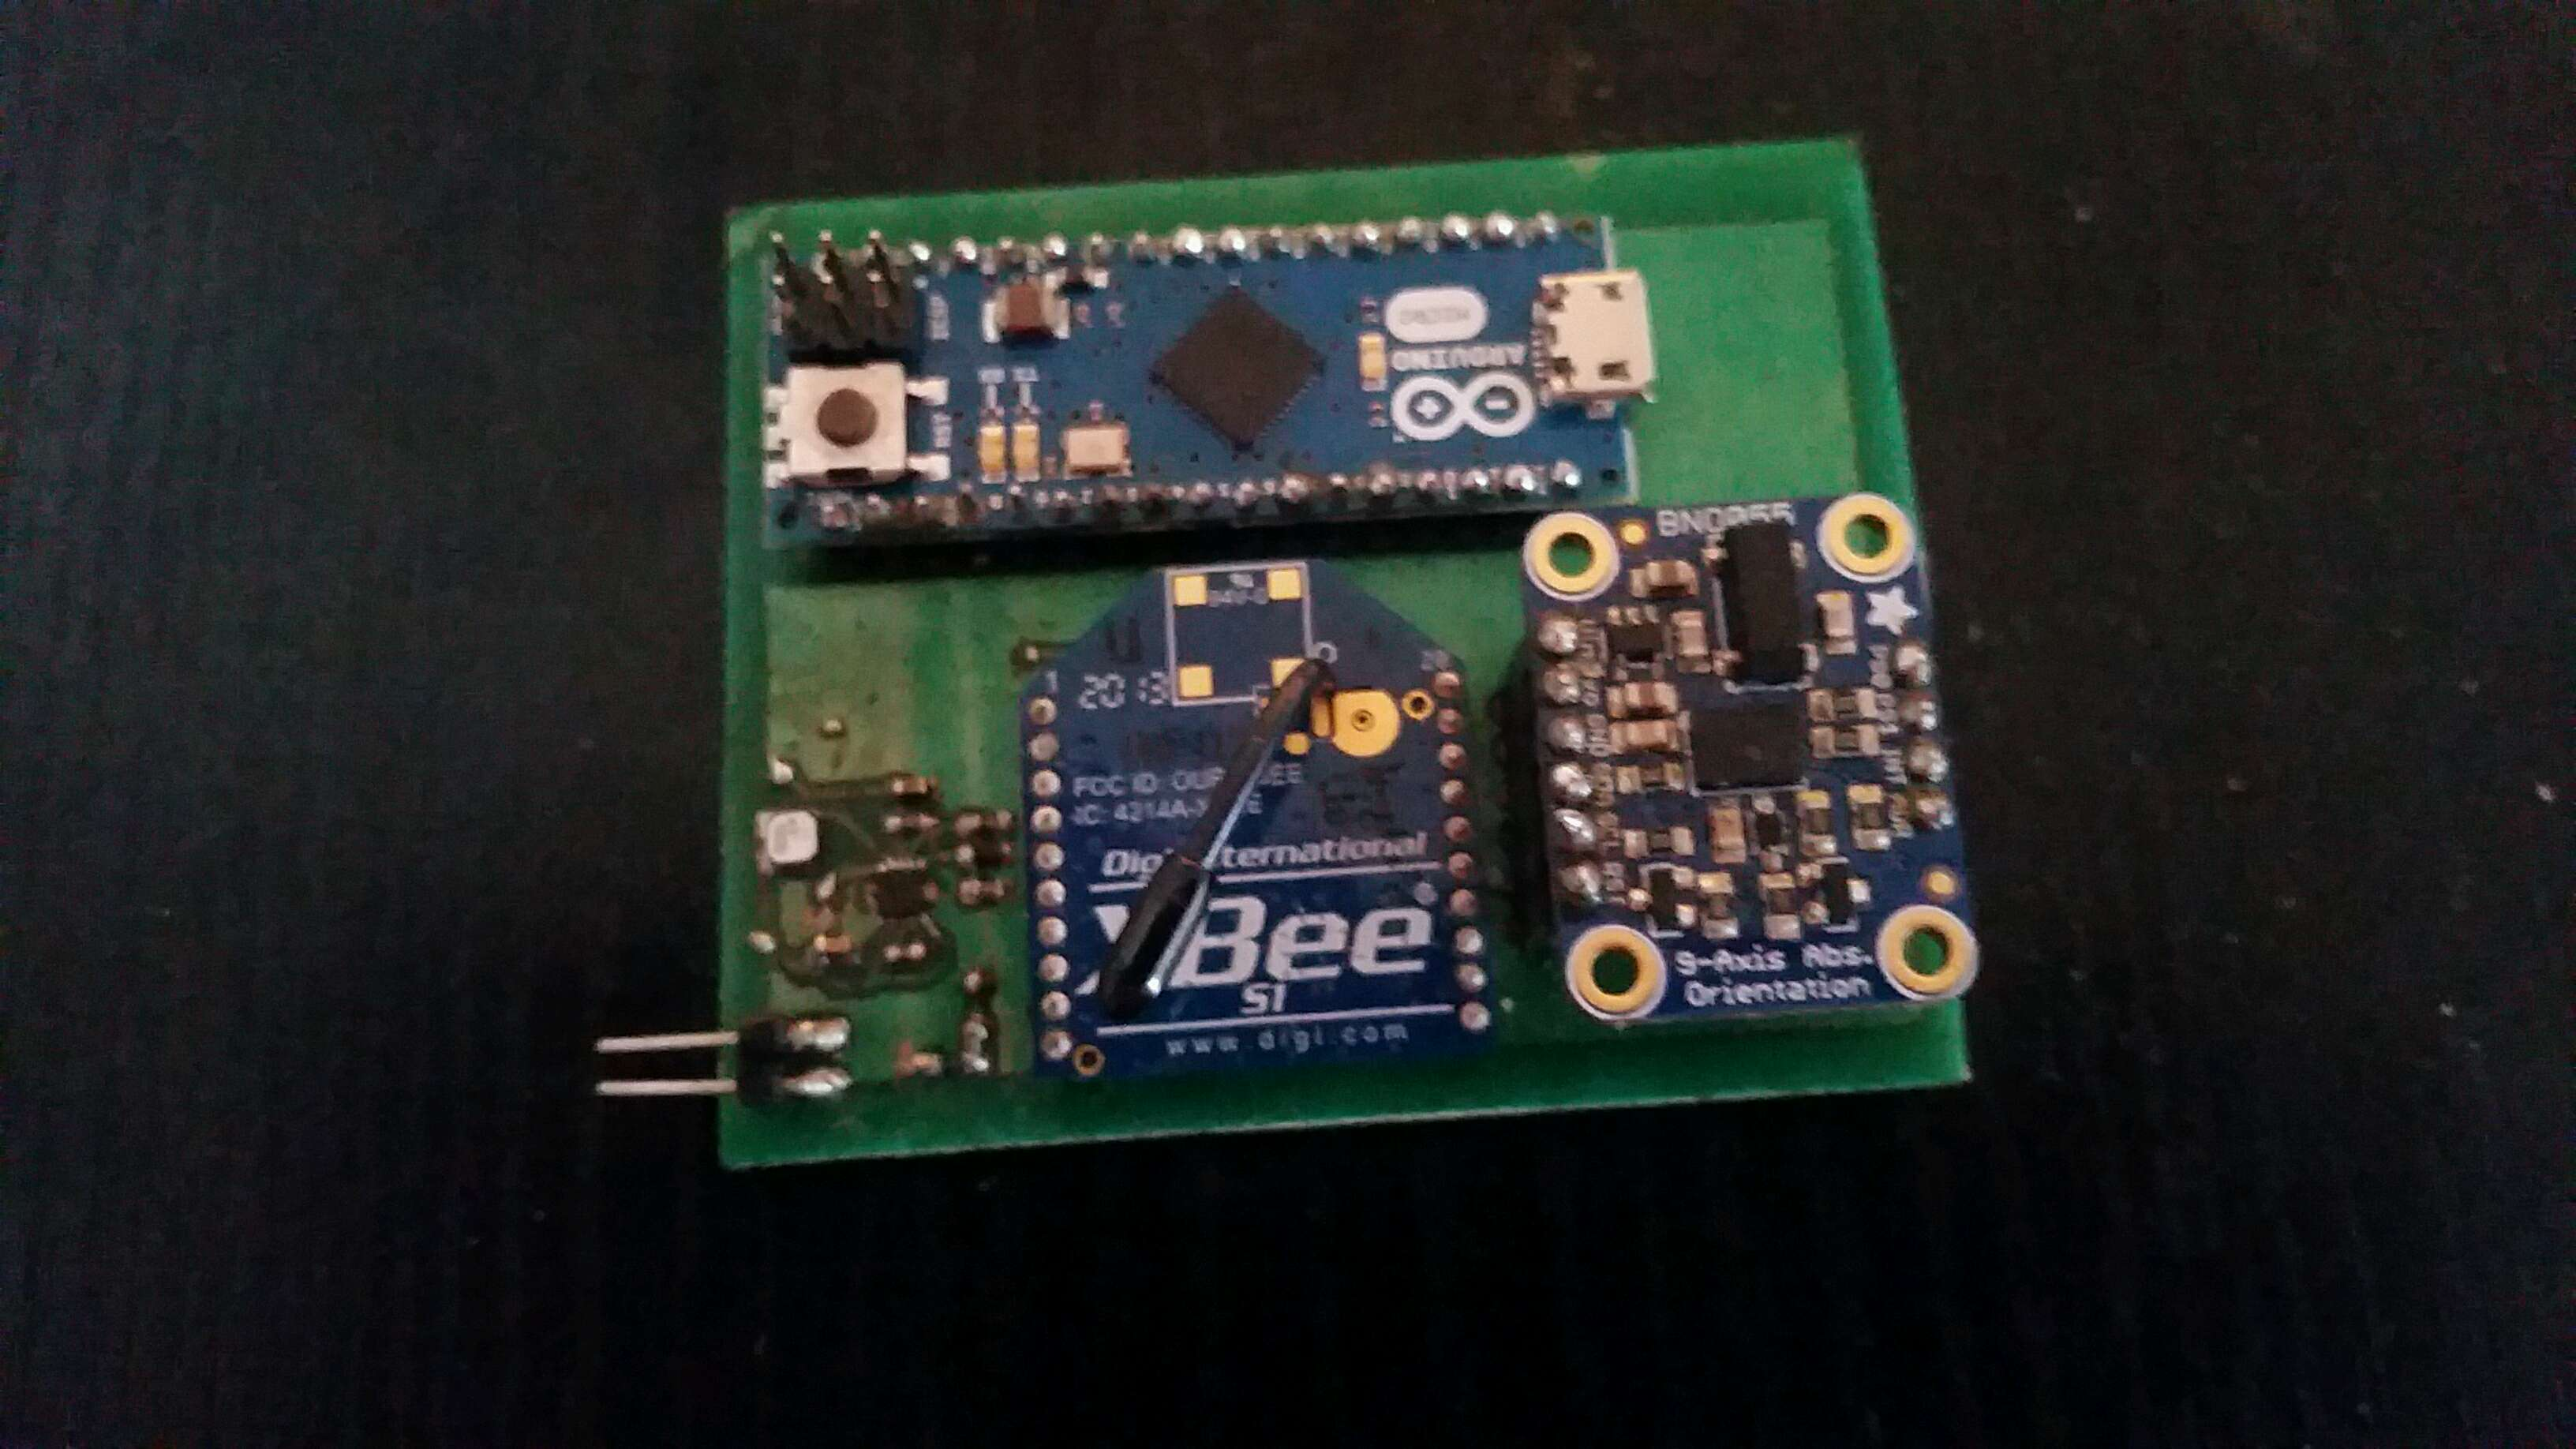
\includegraphics[width=0.4\textwidth]{./pictures/placa1}
		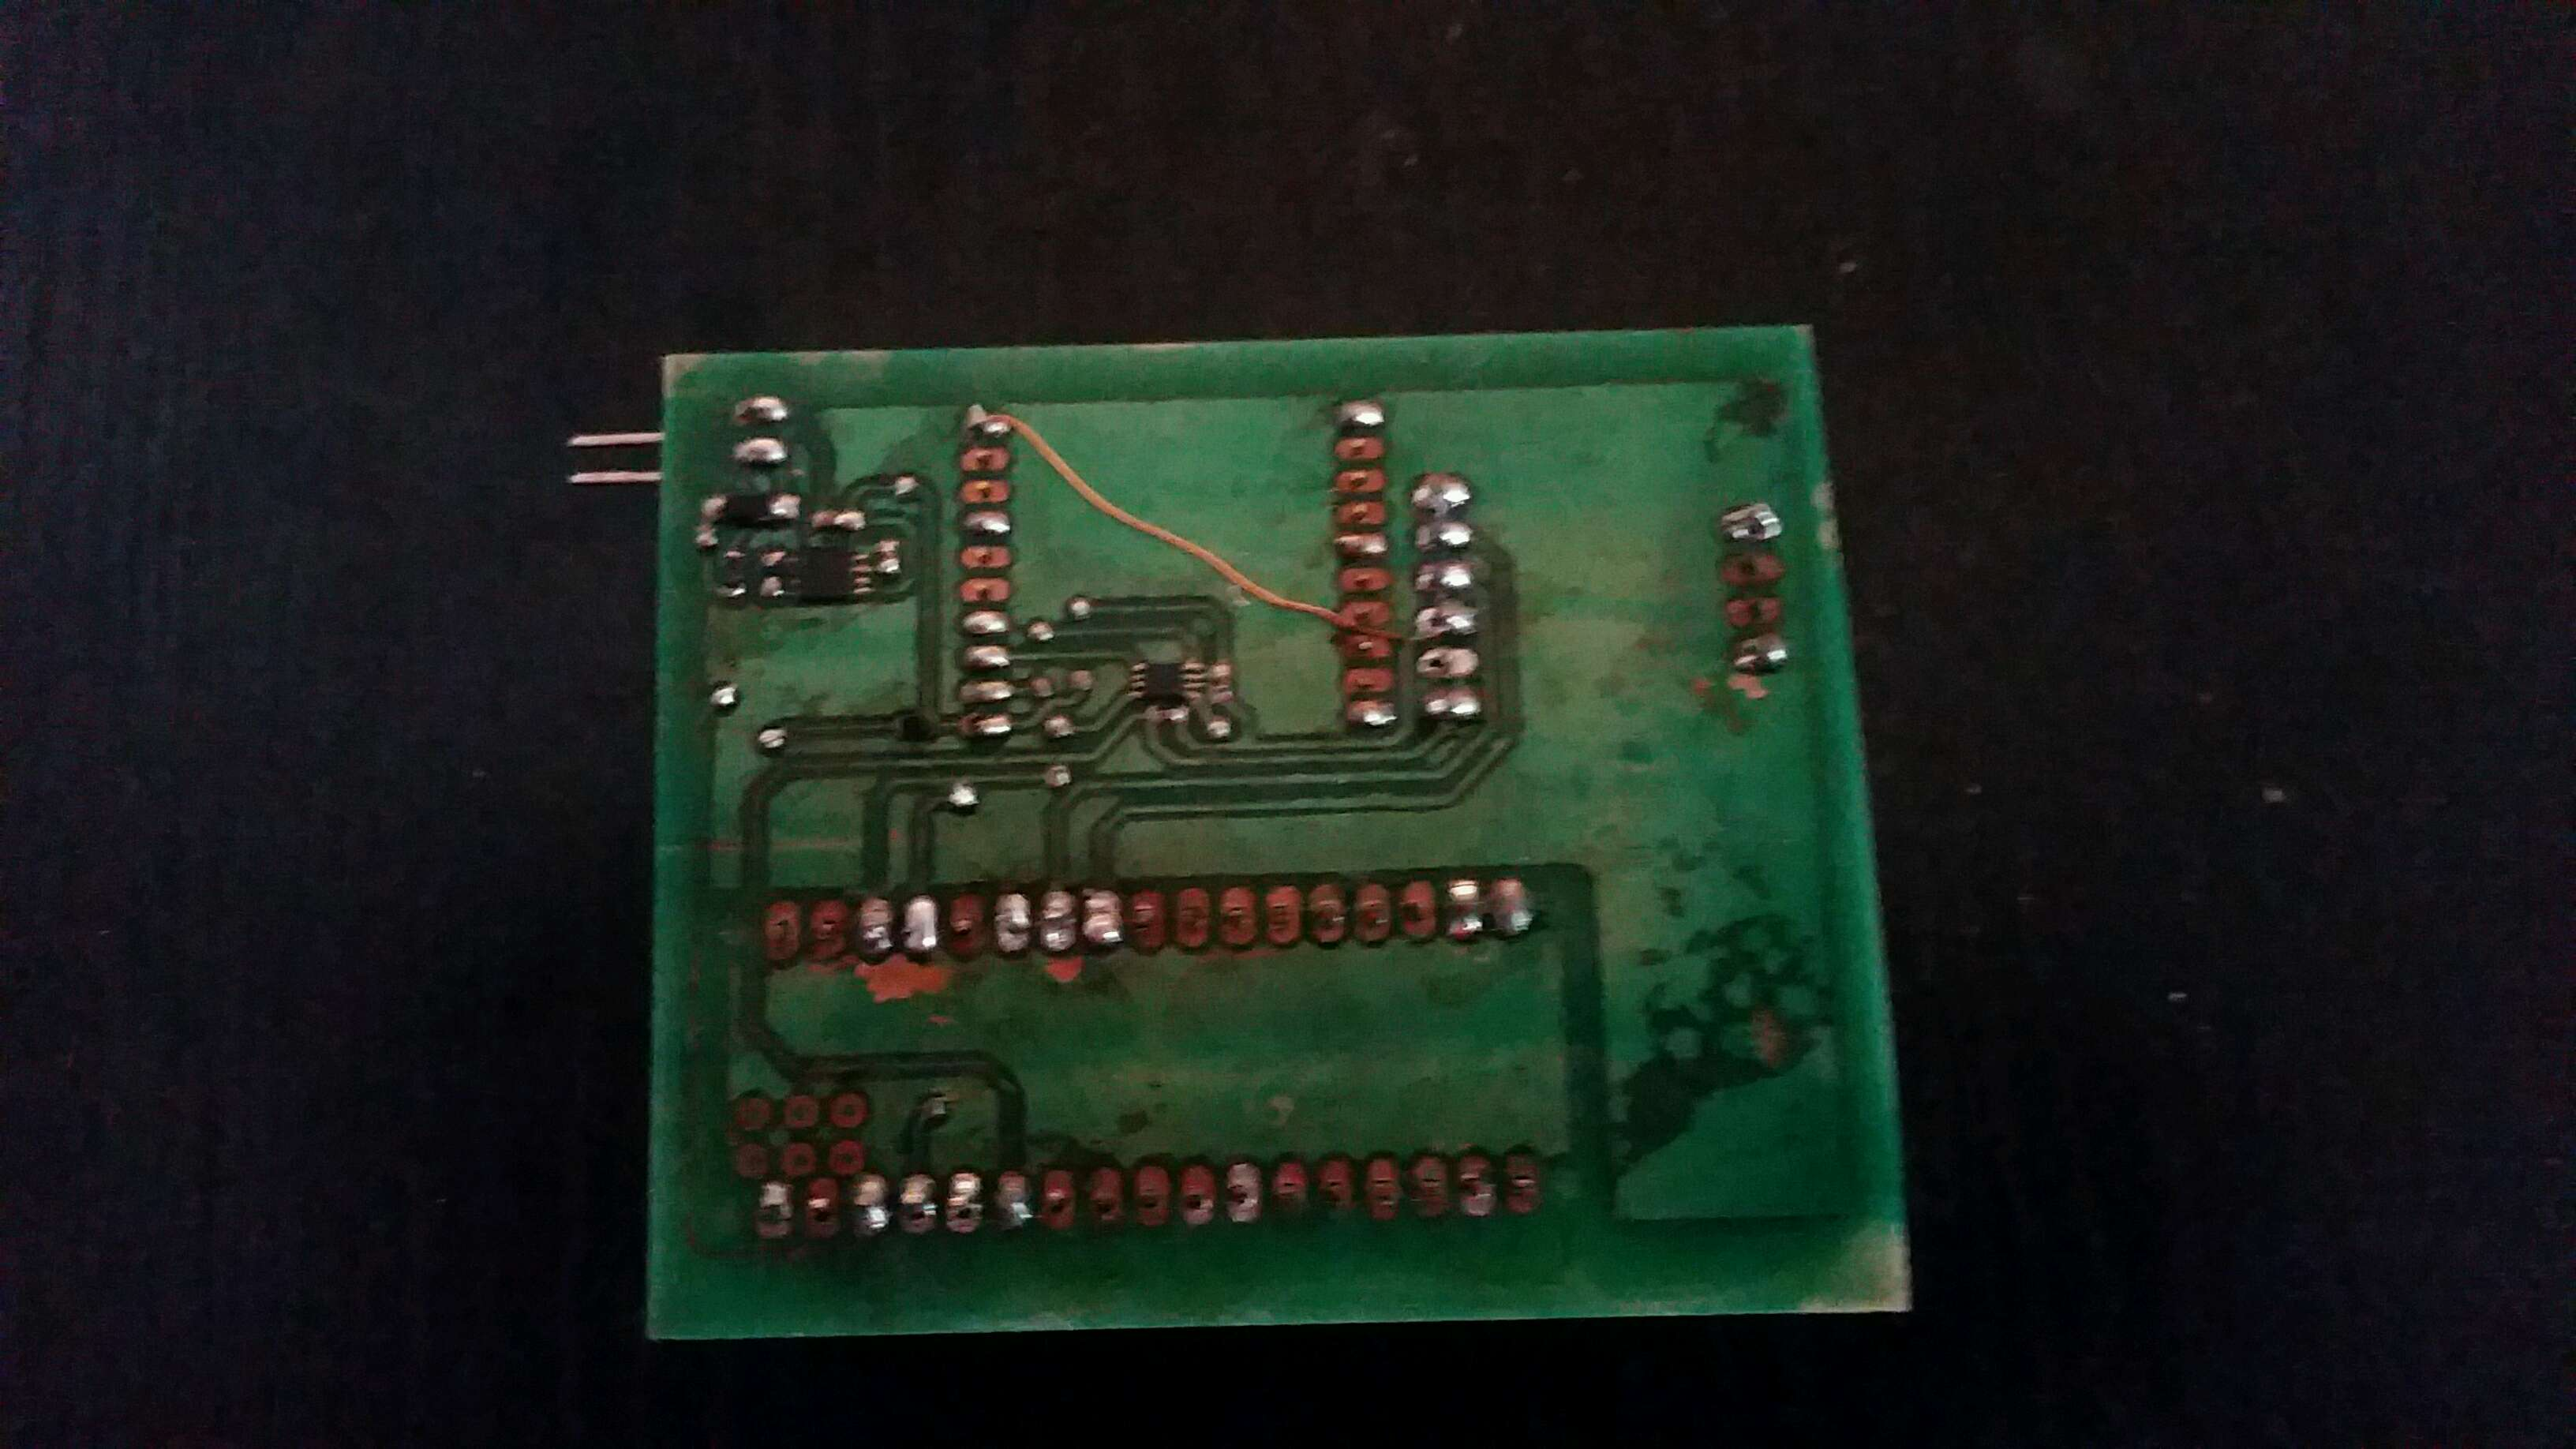
\includegraphics[width=0.4\textwidth]{./pictures/placa2}
	\end{figure}
	\begin{figure}[htbp]
		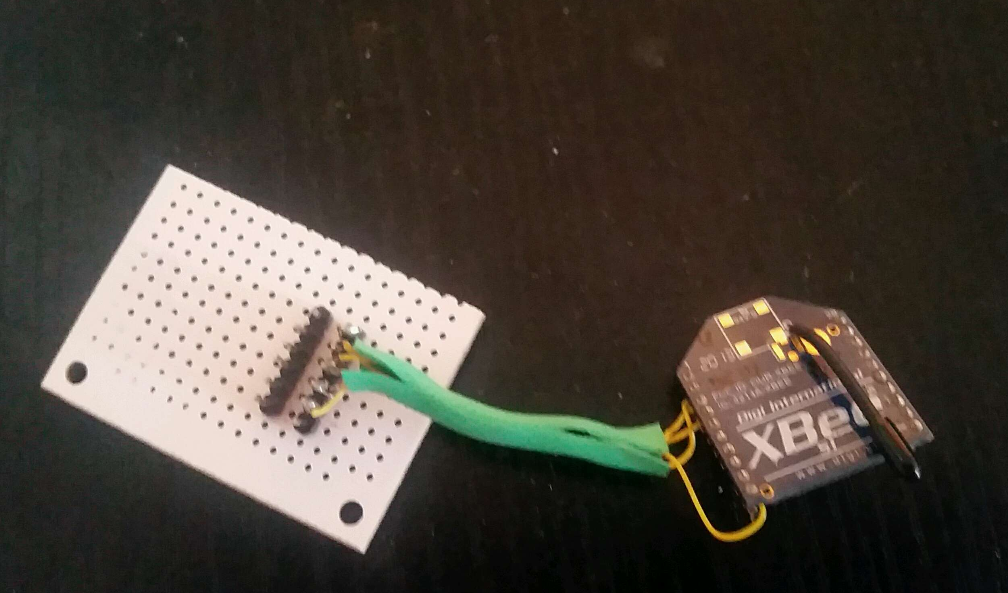
\includegraphics[width=0.4\textwidth]{./pictures/placa3}
		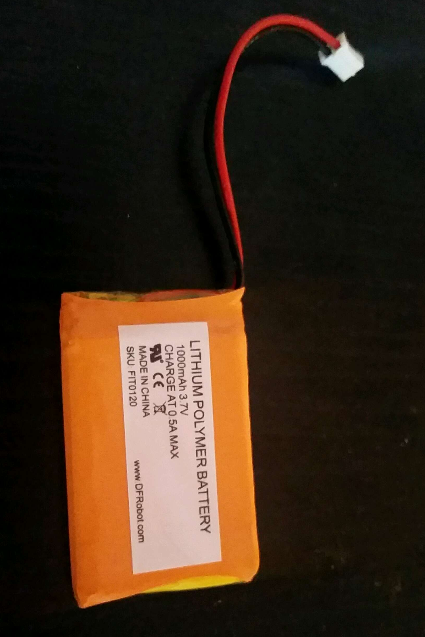
\includegraphics[width=0.2\textwidth]{./pictures/pila}
	\end{figure}
	
\end{frame}	
	
\begin{frame}[fragile]
	\frametitle{Algoritmo generador de mejores posiciones}
	\begin{itemize}
		\item Se toman en cuenta todos los parámetros: W, P, S, L, H...
		\item A cada posición de la figura en pantalla le corresponden dos posiciones en el plano del piso(dos poses de la cabeza)
		\item El algoritmo genera las posiciones en pantalla y en el plano del piso más significativos
		\item El marco de referencia está rotado
	\end{itemize}
	\begin{figure}[htbp]
		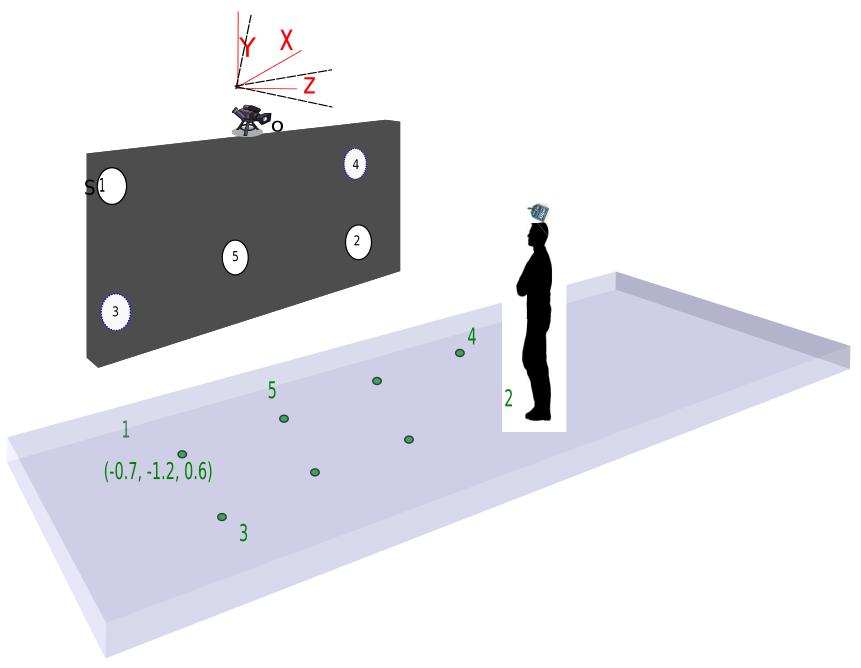
\includegraphics[width=0.7\textwidth]{./pictures/puntos}
	\end{figure}
	
\end{frame}

\begin{frame}[fragile]
	\frametitle{Proyección de puntos en el plano del piso}
El primer paso es conocer dónde se encuentra la cámara con respecto al plano del piso.
	\begin{figure}[htbp]
		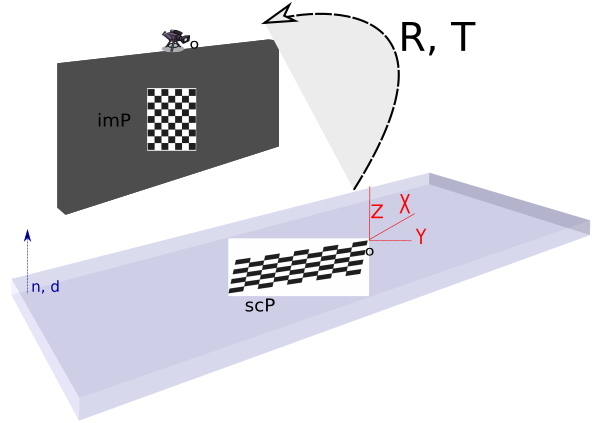
\includegraphics[width=0.65\textwidth]{./pictures/rt}
	\end{figure}
	    {\small\[scP=
	    \begin{bmatrix}
	    0 & 0 & 0.12...\\
	    0 & 0.12 & 0.12...\\
	    0 & 0 & 0...\\
	    1 & 1 & 1... 
	    \end{bmatrix}
	    \]}

\end{frame}

\begin{frame}[fragile]
	\frametitle{Proyección de puntos en el plano del piso}
	\framesubtitle{Descomposición de la homografía}
	\begin{block}{Homografía}
	Es toda transformación proyectiva que determina una correspondencia entre dos figuras geométricas planas
	\end{block}
	A partir de la matriz $H$ y los dos conjuntos de puntos de los planos es posible hallar la matriz de rotación.
	\begin{eqnarray}
	scP_{3x48}=H_{3x3}*imP_{3x48}
	\end{eqnarray}
	
\end{frame}

\begin{frame}[fragile]
	\frametitle{Proyección de puntos en el plano del piso}
	\framesubtitle{Descomposición de la homografía}
	\begin{figure}[htbp]
		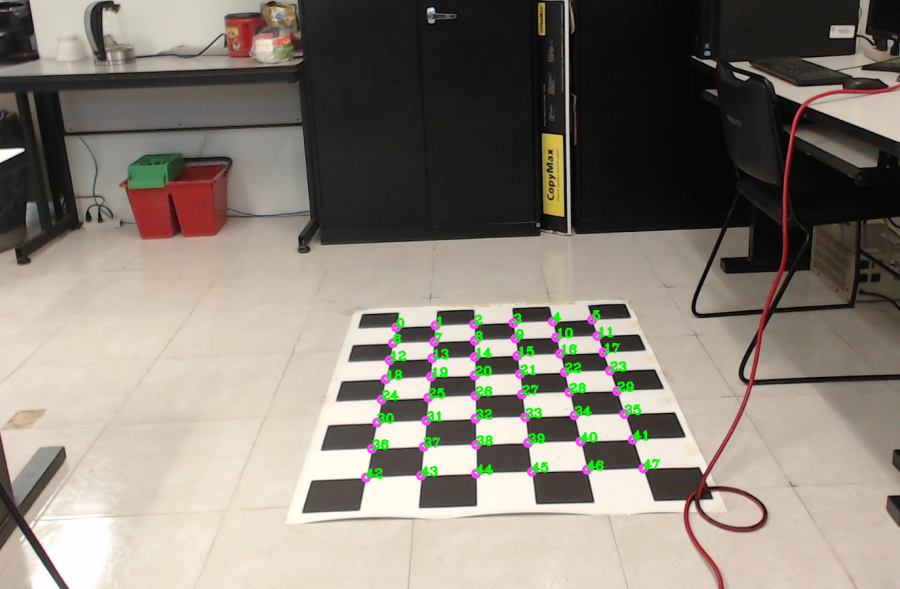
\includegraphics[width=0.65\textwidth]{./pictures/ajedrez}
	\end{figure}
	¿$R$ y $T$ son correctas?
			
\end{frame}

\begin{frame}[fragile]
	\frametitle{Proyección de puntos en el plano del piso}
	\framesubtitle{Plano del piso}
	Conociendo la $R$ y $T$ se calcula la ecuación del plano.
	\begin{figure}[htbp]
		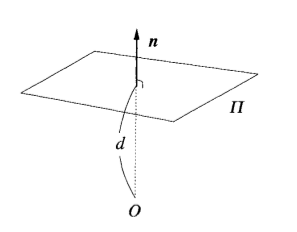
\includegraphics[width=0.3\textwidth]{./pictures/plane}
	\end{figure}
		 \[n=R*\begin{bmatrix}
		 0\\
		 0\\
		 1	
		 \end{bmatrix}\]
		 		\begin{eqnarray}
		 		scPRot_1=R*scP_1+T\\
		 		d=<N,scPRot_1>
		 		\end{eqnarray}
\end{frame}

\begin{frame}[fragile]
	\frametitle{Proyección de puntos en el plano del piso}
	\framesubtitle{Intersección de rectas en el plano}
Verificación de $R$ y $T$ mediante la intersección las rectas de los puntos de la imagen proyectados con el plano del piso
		\begin{figure}[htbp]
			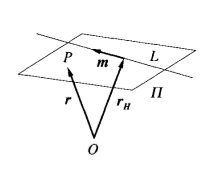
\includegraphics[width=0.3\textwidth]{./pictures/intersec}
		\end{figure}
		\begin{eqnarray}
		r=r_H+\frac{d-<n_{\Pi}, r_H>}{<n_{\Pi},m>}m
		\end{eqnarray}
\end{frame}

\begin{frame}[fragile]
	\frametitle{Proyección de puntos en el plano del piso}
	\framesubtitle{Intersección de rectas en el plano}
	La rotación y traslación calculadas presentan bastante error
	\begin{figure}[htbp]
		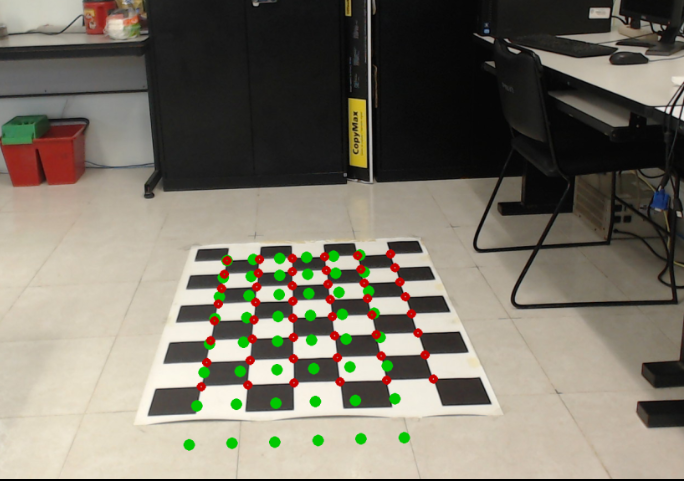
\includegraphics[width=0.6\textwidth]{./pictures/rep}
	\end{figure}	
	Error de 26cm en $X$, 2.68 en $Y$ y 12.8 en $Z$
\end{frame}

\begin{frame}[fragile]
	\frametitle{Optimización numérica de R y T }
%	\framesubtitle{Intersección de rectas en el plano}
\begin{itemize}
	 \item Algoritmo Levenberg–Marquardt
	 \item Miminización de:
 	\begin{eqnarray}
 	F(p)=\frac{1}{2}\sum\limits_1^m(f_i(p))^2	
 	\end{eqnarray}
 	donde $f_i: \mathbb{R}^n\rightarrow \mathbb{R}, i=1,....,m$ son las funciones dadas y $m\geq n$.
 	\item Las funciones a optimizar deben tener los parámetros de $R$ y $T$	
 	\begin{eqnarray}
 	f_{xyz}(p)=||X_{rt}-X_{intersec}||
 	\end{eqnarray}
 	\begin{eqnarray}
 	f_{xyz}(p)= \{R*X_{scn}+T\}-\{ \frac{d}{<n_{\Pi},X_{img}>}X_{img} \}
 	\end{eqnarray}
\end{itemize}
\end{frame}

\begin{frame}[fragile]
	\frametitle{Optimización numérica de R y T}
	En problemas de optimización numérica la redundancia de las matrices de rotación es incoveniente y a menudo es preferible una representación mínima.
	\begin{block}{Fórmula de Rodrigues}
		Cualquier matriz de rotación se puede realizar mediante la rotación
		alrededor de un eje fijo ω por un cierto ángulo $||\omega||$:
	 	\begin{eqnarray}
		 	R=I+\frac{\hat{\omega}}{\parallel\omega\parallel}sin(\parallel\omega\parallel)+ \frac{\hat{\omega}^2}{\parallel\omega\parallel^2}(1-cos(\parallel\omega\parallel))
	 	\end{eqnarray}
	\end{block}
	\begin{eqnarray}
	\begin{array}{c}
	p=[\omega_x, \omega_y, \omega_z, \parallel\omega\parallel, T_x, T_y, T_z]
	\end{array}
	\end{eqnarray}
\end{frame}
\begin{frame}[fragile]
	\frametitle{Optimización numérica de R y T}
	\framesubtitle{Resultados}
	\begin{figure}[htbp]
		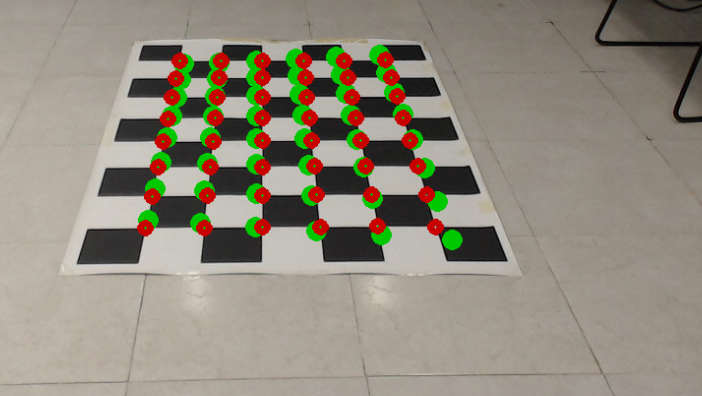
\includegraphics[width=0.6\textwidth]{./pictures/conG0}
	\end{figure}	

\end{frame}
	

%\begin{figure}
%  \centering
%% \includegraphics[width=6cm,height=6cm]{firstex.png}
%\end{figure}


%\section{Metodología}
\begin{frame}[fragile]
\frametitle{Titulo}
%\setbeamerfont{framesubtitle}{subtitulo}
a

\end{frame}
\plain{Questions?}



\end{document}